\documentclass{article}
\usepackage[margin=.9in]{geometry}
\usepackage{xcolor}
\usepackage{subcaption}
\usepackage{amsmath}
\usepackage{amssymb}
\usepackage{float}
\usepackage{listings}
\usepackage{natbib}
\usepackage{booktabs}
\usepackage{listings}
\lstset{
basicstyle=\small\ttfamily,
breaklines=true,
frame=single,
language=Python,
numberstyle=\tiny,
showstringspaces=false
}
\setlength{\parindent}{0pt}
\setlength{\parskip}{\baselineskip}
\definecolor{mycolor}{rgb}{0.1, 0.1, 0.5}
\title{\textcolor{mycolor}{\textbf{{\huge Preliminary Results}}}}
\author{Student: Christopher Hunt \\ Mentor: Dr. Kelsey Stoerzinger}
\date{}
\usepackage{graphicx}
\usepackage{fancyhdr}


\begin{document}
\pagestyle{fancy}
\fancyhf{}
\rfoot{}
\lfoot{Christopher Hunt}
\lhead{Preliminary Results}
\rhead{\thepage}
\maketitle


\subsection*{Results}

During testing of our DIY potentiostat against a BioLogic VSP-300 potentiostat, the measured current response from the working electrode displayed discernible trends. The current fluctuated within the ranges of 0 to 0.4 volts, 0 to 0.5 volts, and 0 to 0.6 volts for scan rates of 20 mV/s, 50 mV/s, and 100 mV/s, respectively (Figure 2). However, a notable disparity emerged when compared to the BioLogic potentiostat's measurements, with the absence of the expected `duck shaped' cyclic voltammogram.

    
The consistency observed in the current response, despite the disparity with the expected cyclic voltammogram, reveals complex dynamics within the potentiostat's function. The discrepancy may point to a limitation or error in the potentiostat design itself. When analyzing the data collected from the DIY potentiostat we see noteable events occuring at approximately 0.07 v, 0.12 v, 0.18 v, 0.23 v, 0.28 v, 0.32 v, 0.38 v, and 0.43 v. These events show characteristics of capacitor charging and rapidly discharging events. This occurs at the near the same potential despite the scan rate. Several factors might have contributed to these unexpected results.

Extensive hardware troubleshooting was conducted. Each signal processing step within the hardware was tested using signals in the expected range of the electrochemical cell. In isolated testing scenarios, the hardware produced the expected values. The success in isolated hardware testing adds complexity to the observed limitation in the current range when connected to the actual electrochemical cell. The divergence between the isolated testing and real-world application highlights a critical area of investigation.

\begin{figure}[H]
  \centering
  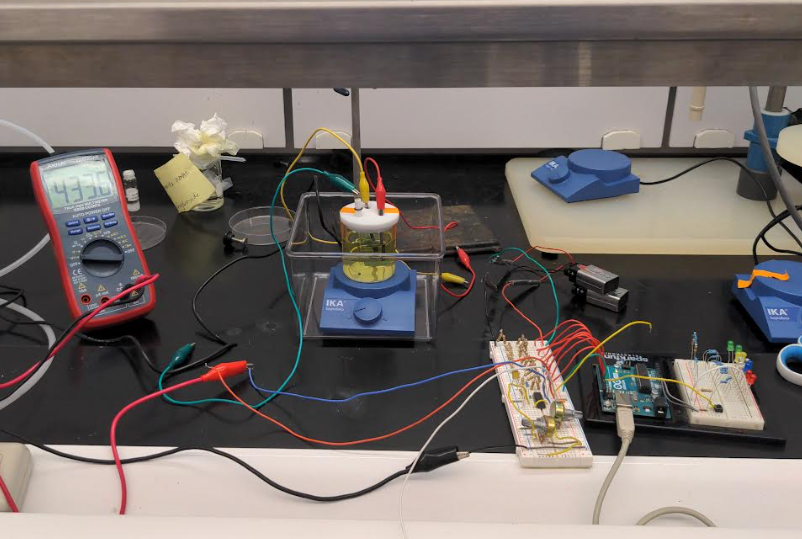
\includegraphics[width=.5\linewidth]{lab_test.png}
  \caption{Ferri/ferrocyanide Redox Reaction Test}
  \end{figure}
  

Though the hardware was designed according to specifications, the observed limitations may stem from several potential sources.
\begin{enumerate}
\item \textbf{Poor Hardware Design}: The entire architecture might not have been optimal for the specific application, leading to inherent limitations.
\item \textbf{Component or Breadboard Issues}: The use of specific components or the breadboard itself might have introduced unexpected behaviors or constraints.
\item \textbf{Choice of Operational Amplifier}: The chosen operational amplifier (LT074 Op Amp) for the design may not have been suitable as the control amplifier.
\end{enumerate}

\begin{figure}[H]
    \centering
    \begin{subfigure}[b]{0.45\textwidth}
    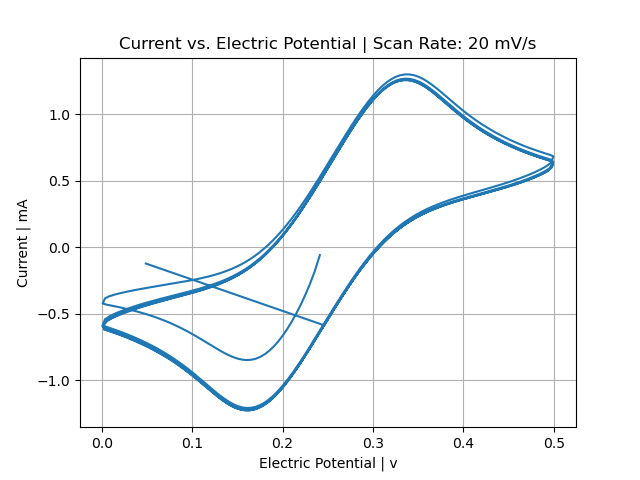
\includegraphics[width=\textwidth]{FECN_20mVs_5cycles_lab.png}
    \caption{BioLogic VSP-300, 20 mV/s, 5 cycles}
    \end{subfigure}
    \hfill
    \begin{subfigure}[b]{0.45\textwidth}
    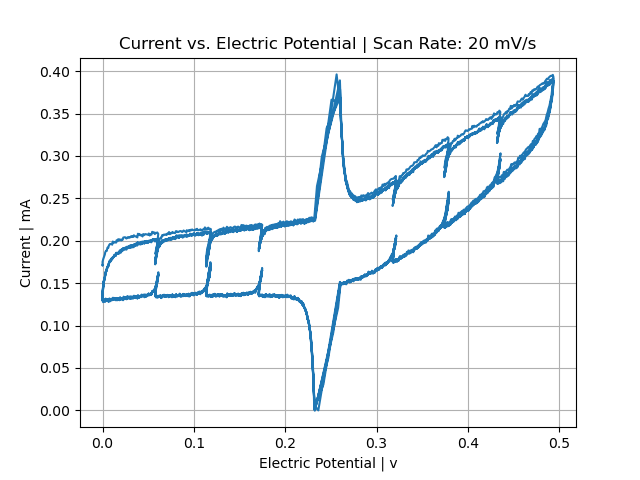
\includegraphics[width=\textwidth]{FECN_20mVs_5cycles.png}
    \caption{DIY Potentiostat, 20 mV/s, 5 cycles}
    \end{subfigure}
    
    \begin{subfigure}[b]{0.45\textwidth}
    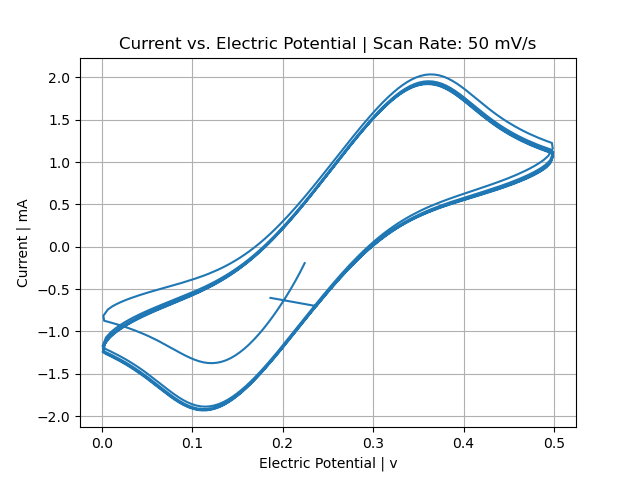
\includegraphics[width=\textwidth]{FECN_50mVs_5cycles_lab.png}
    \caption{BioLogic VSP-300, 50 mV/s, 5 cycles}
    \end{subfigure}
    \hfill
    \begin{subfigure}[b]{0.45\textwidth}
    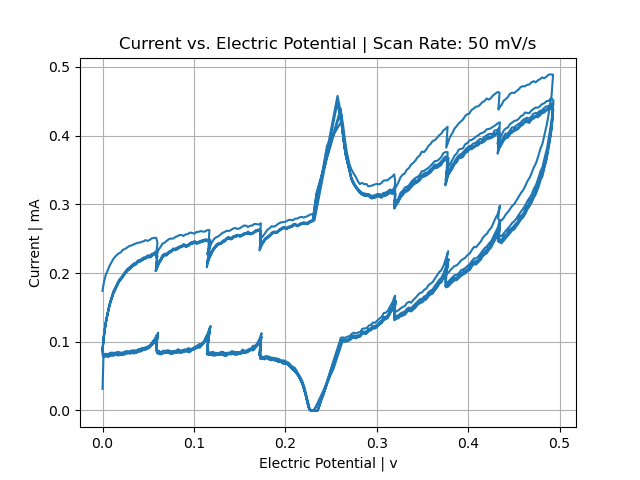
\includegraphics[width=\textwidth]{FECN_50mVs_5cycles.png}
    \caption{DIY Potentiostat, 50 mV/s, 5 cycles}
    \end{subfigure}
    
    \begin{subfigure}[b]{0.45\textwidth}
    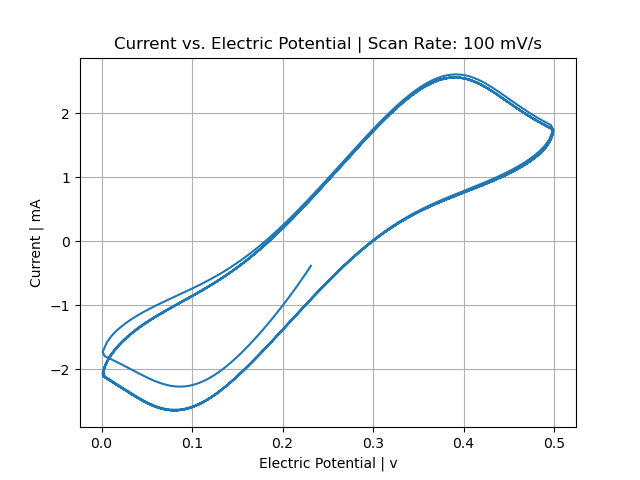
\includegraphics[width=\textwidth]{FECN_100mVs_5cycles_lab.png}
    \caption{BioLogic VSP-300, 100 mV/s, 5 cycles}
    \end{subfigure}
    \hfill
    \begin{subfigure}[b]{0.45\textwidth}
    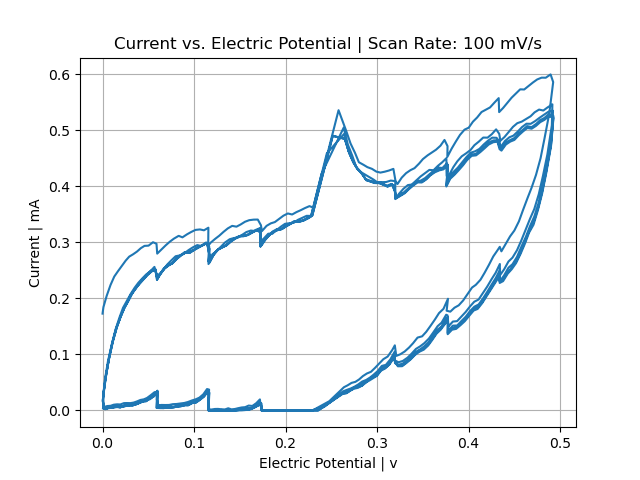
\includegraphics[width=\textwidth]{FECN_100mVs_5cycles.png}
    \caption{DIY Potentiostat, 100 mV/s, 5 cycles}
    \end{subfigure}
    \caption{Cyclic voltammograms comparison}
    \end{figure}

The multifaceted nature of the potential errors presents a challenge in pinpointing the exact cause. Further detailed analysis and redesign may be required to isolate and rectify the underlying issues. The findings from this study provide valuable insights into the complexities of custom potentiostat design. While the observed trends and successful isolated testing demonstrate a degree of functionality, the disparity with expected results points to critical areas for improvement.

Further investigation into the specific components, hardware design, and choice of operational amplifier is warranted. Future work should focus on systematically evaluating each potential source of error, leading to refined designs and potentially unveiling insights into potentiostat function.



Despite existing errors in our DIY potentiostat design, this research highlights potential success with our expressed goal of developing educational materials and tools. With further time and assistance from electrical engineering professionals, achieving a DIY design that rivals lab-grade instruments may be possible.


\end{document}

